\label{chap:discussion}

This chapter combines the findings from the DSPI analysis and the qualitative text classification to address the research questions. The results are interpreted using Business Model Innovation (BMI) theory.

\section{Strategic Archetypes}
Based on the Terms of Service analysis ($N=8$), we identify three distinct strategies that digital firms use:

\subsection{The Content Fortress: Defensive Value Capture}
Firms adhering to this strategy, typified by streaming giants like \textbf{Netflix} and \textbf{Disney+}, prioritize the integrity of their **Value Capture** mechanism (market segmentation) over the frictionless nature of their **Value Delivery**. Our quantitative analysis reveals that within the "Content Licensing Sector," the specific correlation between price variance and enforcement is negative ($R \approx -0.47$). This indicates that strict enforcement is not a *reaction* to specific price arbitrage risks, but an \textbf{industry standard}—a baseline requirement for asserting their Value Proposition (exclusive content) in specific regions. \textbf{Disney+} and \textbf{Netflix} allocate approximately \textbf{8.5\%} and \textbf{6.2\%} of their enforcement clauses to \textbf{Content Licensing} issues, respectively.

This aligns with the "Fortress" strategy described by \textcite{schmidt2020transnational}, where incumbent firms construct digital barriers to protect legacy revenue streams. However, as noted by \textcite{lobato2019geoblocking}, such strategies often suffer from a "legibility" problem—users encounter "This content is not available" error messages without understanding the underlying legal framework.

\subsection{The Ecosystem Fortress: Adaptive Value Proposition}
Platforms like \textbf{Apple Music} exemplify a "Globalist" approach that innovates on the **Value Proposition**. With almost no focus on \textbf{Technical Blocking} (0.15\%) and a strong emphasis on \textbf{Price Discrimination} (5.7\%), Apple appears to accept the reality of international fragmentation \parencite{brouthers2016explaining}. Rather than "repairing" the Value Capture mechanism through blocking, they rely on a superior Value Delivery ecosystem (hardware integration, iCloud) that makes the friction of using a VPN-based "foreign" account essentially "not worth it" for the user.

\subsection{The Enterprise Fortress: Identity-Based Value Capture}
A new archetype identified in this study is the "Enterprise Fortress," exemplified by \textbf{Microsoft}. Despite having the lowest global price variance in the dataset (indicating a relatively harmonized global price for Microsoft 365), Microsoft exhibits the highest intensity of "Account Action" clauses. This suggests that for utility software, the **Value Capture** is protected not by *network* blocking (which targets Location), but by *identity* verification (which targets the User). The "Fortress" is built to keep unauthorized resellers out, reinforcing the subscription model's integrity without compromising the global **Value Delivery** of the software itself.

\subsection{The Utility Paradox (Adobe)}
\textbf{Adobe} presents a unique case. It has high price discrimination (similar to Netflix) but relatively low ``Technical Blocking'' enforcement. Based on our analysis of Adobe's Terms of Service and product documentation, this appears to be because Adobe's enforcement mechanism is ``on-device'' (software activation keys) rather than ``on-network'' (IP filtering). This observation suggests that ``Technical Blocking'' is a strategy specific to \textit{cloud-streamed} content, whereas \textit{downloaded software} may rely on different protection mechanisms.

However, a hybrid future appears to be emerging in the form of \textbf{"Always-Online DRM"}. Features like Adobe's cloud-dependent generative tools require authenticated connections to function, effectively merging network-based verification with identity authentication. This reflects the "Opportunities and Risks" of SaaS adoption \parencite{benlian2011opportunities}, where control shifts from the client device to the cloud provider.
\subsection{The Adversarial Cycle: A Longitudinal View}
The relationship between providers and consumers is not static. Our historical analysis reveals a clear "Action-Reaction" cycle, visualized in Figure \ref{fig:timeline}.

\begin{figure}[ht]
    \centering
    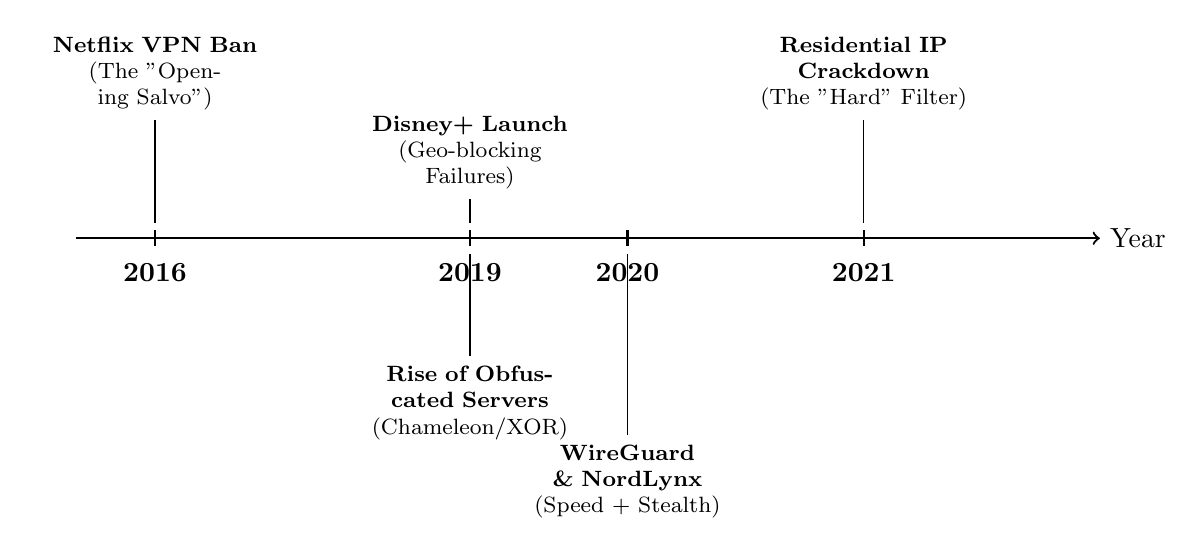
\begin{tikzpicture}[x=2cm, y=1cm]
        % Draw the timeline line
        \draw[->, thick] (0,0) -- (6.5,0) node[right] {Year};
        
        % Ticks and Labels
        \foreach \x/\year in {0.5/2016, 2.5/2019, 3.5/2020, 5.0/2021} {
            \draw[thick] (\x,0.1) -- (\x,-0.1);
            \node[below=0.2cm] at (\x,0) {\textbf{\year}};
        }

        % Events Top (Corporate/Coercive)
        \node[align=center, text width=3cm, above=1.5cm, font=\footnotesize] (netflix16) at (0.5,0) {\textbf{Netflix VPN Ban}\\(The "Opening Salvo")};
        \draw[thin] (0.5,0.2) -- (netflix16);

        \node[align=center, text width=3cm, above=0.5cm, font=\footnotesize] (disney19) at (2.5,0) {\textbf{Disney+ Launch}\\(Geo-blocking Failures)};
        \draw[thin] (2.5,0.2) -- (disney19);
        
        \node[align=center, text width=3cm, above=1.5cm, font=\footnotesize] (resip) at (5.0,0) {\textbf{Residential IP Crackdown}\\(The "Hard" Filter)};
        \draw[thin] (5.0,0.2) -- (resip);

        % Events Bottom (VPN/Adaptive)
        \node[align=center, text width=3cm, below=1.5cm, font=\footnotesize] (obfus) at (2.5,0) {\textbf{Rise of Obfuscated Servers}\\(Chameleon/XOR)};
        \draw[thin] (2.5,-0.2) -- (obfus);

        \node[align=center, text width=3cm, below=2.5cm, font=\footnotesize] (wireguard) at (3.5,0) {\textbf{WireGuard \& NordLynx}\\(Speed + Stealth)};
        \draw[thin] (3.5,-0.2) -- (wireguard);

    \end{tikzpicture}
    \caption{The Adversarial Timeline: Coercive Barriers vs. Technical Circumvention.}
    \label{fig:timeline}
\end{figure}

This timeline illustrates the dynamic relationship between corporate enforcement and consumer behavior. Following the 2016 Netflix enforcement measures, VPN providers developed "Obfuscated Servers" (circa 2019), which subsequently led to more sophisticated blocking techniques (circa 2021). This pattern suggests an ongoing adaptation process on both sides \parencite{hohn2021vpn}.

\section{Limitations and Validity}
While this study provides a new quantitative framework for analyzing geo-arbitrage, several limitations must be noted to put the findings in context.

\subsection{Sample Size and Generalizability}
The correlation analysis relies on a strategic sample of $N=8$ major digital service providers. While these firms represent a significant majority of the consumer subscription market by capitalization, the sample is small in statistical terms. Consequently, the findings should be interpreted as "exploratory" evidence of strategic archetypes rather than a definitive "law" of digital economics. Future research could expand this dataset to include mid-tier SaaS providers to test if the "Enterprise Fortress" model holds for smaller B2B firms.

\subsection{The "Average Citizen" Bias (Socioeconomic Mismatch)}
Our "Affordability" metric calculates cost as a percentage of the \textit{Average National Monthly Wage}. However, in emerging markets like Turkey or Argentina, the target demographic for services like Netflix or Adobe is likely the urban upper-middle class, whose income is significantly higher than the national average. 

For instance, World Bank data and local surveys indicate that in Turkey, the top 20\% of earners capture nearly 48\% of total disposable income. Similarly, in Argentina, the top 10\% of earners have average monthly incomes exceeding \$496 USD, well above the national median. This implies that global digital services are aggressively priced to target this specific "Global Elite" segment. As \textcite{kastanakis2012between} argue, in markets with high income inequality, luxury consumption (including premium digital subscriptions) serves as a critical status signal for the upper class. This "Elite Targeting" pricing strategy explains why firms tolerate some level of piracy from the lower 80\%—they were never the primary customer segment to begin with.

The Digital Services Price Index (DSPI) represents a snapshot of pricing data from late 2024 to early 2025. In hyperinflationary economies such as Argentina and Turkey (both classified as hyperinflationary under IAS 29), local currency prices are adjusted frequently in response to macroeconomic conditions. A ``cheap'' arbitrage opportunity identified in this thesis could be eliminated by a price adjustment or currency devaluation. The ``Arbitrage Window'' is therefore dynamic rather than static.

\subsection{AI Classification Reliability}
The use of Large Language Models (Gemini 3 Flash) creates a potential "Black Box" validity risk. To reduce this, we used the model's self-reported confidence scores as a filtering mechanism. The final dataset achieved an average confidence score of \textbf{0.947}, with \textbf{80.5\%} of classifications exceeding a confidence threshold of 0.9. This high degree of certainty suggests that the detection of "coercive" vs. "general" language is reliable, even without human verification for every datapoint.

\subsection{A Methodological Finding: BERT Models and Legal Text}
Beyond the primary research findings, this study contributes a methodological insight: traditional BERT-based Natural Language Inference models are inadequate for complex legal text classification in the domain of Terms of Service analysis. The comparative evaluation (see Section \ref{sec:llm_methodology}) showed that Zero-Shot BERT achieved only \textbf{26.8\%} agreement with the validated Gemini classifications, with a Cohen's Kappa of \textbf{0.032}—effectively random chance.

This poor performance stems from the fundamental difference between keyword matching and semantic reasoning. BERT models flag sentences based on surface-level keyword presence (e.g., marking "You must have an account" as "Account Action"), while LLMs with larger context windows can distinguish between routine legal boilerplate and actual enforcement clauses. This finding suggests that future research in computational legal analysis should prioritize modern generative models over traditional NLI approaches when dealing with nuanced, domain-specific language.
